\documentclass{beamer}
\renewcommand{\baselinestretch}{1.1}
\usepackage{graphicx}
\usepackage{natbib}
\usepackage{amsmath}
\usepackage{hyperref}
\usepackage{listings} 

\def\labelitemi{--}
\parindent=0pt

\usepackage{xcolor}

\colorlet{codecolor}{black!30}
\newcommand{\codebox}[1]{%
  \colorbox{codecolor}{\ttfamily \detokenize{#1}}%
}

\begin{document}


{\usebackgroundtemplate{%
  \includegraphics[width=\paperwidth,height=\paperheight]{images/Dec07_SW_Ero&Flower_99sm.jpg}} 
\begin{frame}
\begin{center}
\vspace{-20ex}
{\color{white} {\huge USDA/EGRET model}}
\\
\vspace{0ex}
{\color{white} {\Large 30 September 2026}}

\end{center}
\end{frame}
}

	\frame{
		\frametitle{Overall question: How does temperature affect germination?}
}

	\frame{
		\frametitle{Overall question: How does temperature affect germination?}
			\begin{itemize}
			\item What are the average overall responses to chilling and forcing? 
			\item And how does it vary by species? (And what is $\lambda$?)
			\item And dormancy classes?
			\end{itemize}
	}
	

		\frame{
		\frametitle{How the model works}
		\framesubtitle{Grab from provenance model?}
			\begin{align*}
			\hat{y} & = \alpha_0 + \alpha_{provenance} + \beta (C) \\ % percent germination!
			\alpha_{provenance} & \sim MVN(0, \sigma_{\alpha}^2)\\
			y & \sim normal(\hat{y}, \sigma_y^2)\\
			\end{align*}
	}

	\frame{
		\frametitle{Results so far ... forcing/chilling}
		\framesubtitle{Overall: Gymnosperms vs. angiosperms}
		\noindent \includegraphics[width=0.6\textwidth]{} 
	}
	
		\frame{
		\frametitle{Results so far ... forcing/chilling and intercept}
		\framesubtitle{Overall: Gymnosperms vs. angiosperms}
		\noindent \includegraphics[width=0.6\textwidth]{} 
	}
	
		\frame{
		\frametitle{Results so far ... forcing/chilling}
		\framesubtitle{Phylogenetic effects: intercept, chilling, forcing (angio and gymno)}
		\noindent 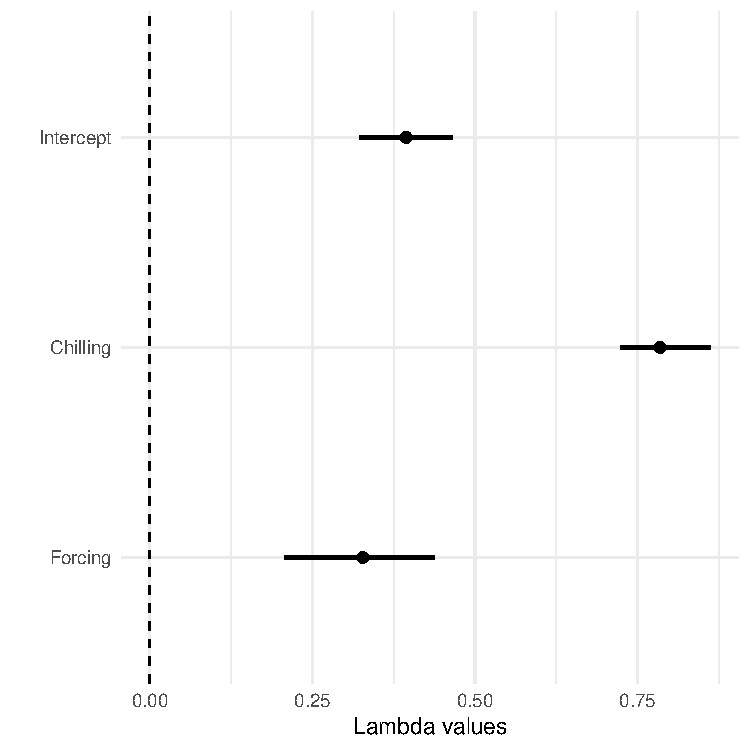
\includegraphics[width=0.6\textwidth]{..//..//analyses/analyseBudSeed/figures/lambdaAngio.pdf} 
	}
	
			\frame{
		\frametitle{Results so far ... forcing/chilling}
		\framesubtitle{Many species!}
		\noindent \includegraphics[width=0.6\textwidth]{} 
	}
	
		
			\frame{
		\frametitle{Results so far ... forcing/chilling}
		\framesubtitle{Dormancy classes}
		\noindent \includegraphics[width=0.6\textwidth]{} 
	}
	
		\frame{
		\frametitle{Other things we should look at?}
	}
	
			\frame{
		\frametitle{Other things we should look at?}
		\begin{itemize}
			\item Seed size?
			\end{itemize}
	}
	

	


\end{document}